% Template for ICASSP-2013 paper; to be used with:
%          spconf.sty  - ICASSP/ICIP LaTeX style file, and
%          IEEEbib.bst - IEEE bibliography style file.
% --------------------------------------------------------------------------



% ++++++++++++++++++++++++++++++++++++++++++++++++++++++++++++++++++++++++++++++
% + Document preamble
\documentclass{article}


% Packages
% --------
\usepackage{spconf,amsmath,graphicx}
\usepackage[total={178mm,229mm},top=25mm,left=19mm]{geometry}
\usepackage{amssymb}
\usepackage{bm}
\usepackage[font=small,labelfont=bf]{caption}
\usepackage{subcaption}
\usepackage{cite}
\usepackage{soul}
\usepackage{algorithm}
\usepackage{algorithmic}

% Definitions
% -----------
\def\x{{\mathbf x}}
\def\L{{\cal L}}

% Mathematical tips
\providecommand{\abs}[1]{\lvert#1\rvert}
\providecommand{\norm}[1]{\lVert#1\rVert}
\providecommand{\red}[1]{\textcolor{red}{#1}}

% Tikz commands
\usepackage{tikz}
\usepackage{mathabx}
\usepackage{geometry}
\usetikzlibrary{arrows,chains,matrix,positioning,scopes,calc,fit}
\tikzset{
  empty/.style={draw=none, fill=none},
  rect/.style={shape=rectangle},
  rectRound/.style={shape=rectangle, rounded corners},
  greyDotted/.style={draw=black!50!white, dash pattern=on 1pt off 4pt on 6pt off 4pt, inner sep=2mm, rectangle, rounded corners}
}
\newcommand{\DeltaTrain}{
  \draw[rounded corners, dashed] (-1cm,-2mm) rectangle (1cm,1cm);
  \draw[->] (-6mm,0) -- (-6mm,4mm);
  \draw[->] (0,0) -- (0,8mm);
  \draw[->] (4mm,0) -- (4mm,5mm);
  \draw[->] (6mm,0) -- (6mm,7mm);
  \draw (-9mm,0) -- (9mm,0);
  \node[empty, minimum width=2.4cm, minimum height=1cm]{};
}
\newcommand{\Sampling}{
  \coordinate (A) at (-2.4mm,0mm);
  \coordinate (B) at (2.4mm,0mm);
  \coordinate (P) at ($(A) + (45:4.8mm)$);
  \coordinate (Q) at ($(A) + (80:2.5mm)$);
  \draw (A) -- (P);
  \draw[->] (Q) arc (95:-25:2.5mm);
  \draw node[empty,above] at (P) {\scriptstyle t=nT};
  \node[empty, minimum width=4.8mm]{};
}

% Algorithmic package, rename "Require/Ensure" into "Input/Output"
\renewcommand{\algorithmicrequire}{\textbf{Input:}}
\renewcommand{\algorithmicensure}{\textbf{Output:}}


% - end of document preamble
% ------------------------------------------------------------------------------



% ++++++++++++++++++++++++++++++++++++++++++++++++++++++++++++++++++++++++++++++
% + Beginning of content
\begin{document}


% Title, authors and address
% --------------------------
\title{Sequential local FRI sampling of infinite streams of Diracs}

\name{Jon O\~{n}ativia, Jose Antonio Urig\"{u}en and Pier Luigi Dragotti 
\thanks{This work was supported by the European Research Council (ERC)
starting investigator award Nr. 277800 (RecoSamp).}}
\address{Department of Electrical and Electronic Engineering,
Imperial College London, UK\\
\normalsize \texttt{\{ jon.onativia, jose.uriguen08, p.dragotti \} @imperial.ac.uk}
}

\maketitle


% Abstract and keywords
% ---------------------
\begin{abstract}
The theory of sampling signals with finite rate of innovation (FRI) has shown 
that it is possible to perfectly recover classes of non-bandlimited signals
such as streams of Diracs from uniform samples. Most of previous papers, 
however, have to some extent only focused on the sampling of periodic or 
finite duration signals. 

In this paper we propose a novel method that is able to reconstruct infinite 
streams of Diracs, even in high noise scenarios.
We sequentially process the discrete samples and output locations and amplitudes
of the Diracs in real-time.
We first establish conditions for perfect reconstruction in the noiseless case
and then present the sequential algorithm for the noisy scenario.
We also show that we can achieve a high reconstruction accuracy of $1000$ Diracs 
for SNRs as low as 5dB.
\end{abstract}

\begin{keywords}
Analog-to-digital conversion, finite rate of innovation, sampling theory,
annihilating filter.
\end{keywords}


% Introduction
% ------------
\section{Introduction}
\label{sec:intro}

Streams of Diracs are  the canonical example of signals with finite rate of innovation 
(FRI) in that they are completely specified by a finite number of parameters per unit of time. 
Periodic streams of Diracs are sampled and perfectly reconstructed in 
\cite{vetterli2002} using the sinc kernel.  
Authors in \cite{dragotti2005,dragotti2007} instead propose the use of kernels that reproduce 
polynomials or exponentials and also propose a sequential algorithm 
to sample and perfectly reconstruct infinite streams of Diracs. The sequential algorithm, 
however,  was designed to deal only with noiseless samples.
The family of sum of sincs (SoS) kernels was introduced in \cite{tur2011} 
for the sampling of periodic stream of pulses such as Diracs, authors also consider the
case of infinite streams of Diracs. However, their method requires that the 
stream of Diracs be `bursty'. Specifically, a group of $K$ Diracs must be followed
by a long period of absence of Diracs in order for the method to work. 
They also assume that the reconstruction algorithm is synchronised with the sampling process in order to 
be automatically in phase with the time window containing the burst of Diracs.

In this paper we propose a novel 
approach to reconstruct infinite streams of Diracs, in high 
noise scenarios, with no clear separation between bursts. 
We sequentially process the discrete samples and output locations and amplitudes
of the Diracs in real-time.
We first establish conditions for perfect reconstruction in the noiseless case
and then present the sequential algorithm for the noisy scenario.
We show through simulations  that the algorithm is able to process $10000$ 
samples in about $100$ seconds and that it can retrieve with high accuracy 
$1000$ Diracs even in very low SNR regimes.

The paper is organised as follows. In Section \ref{sec:sampling} 
we review the case of sampling and reconstructing a finite stream of $K$ 
Diracs as presented in \cite{dragotti2007}. 
In Section \ref{sec:inf_stream} we explain our 
sequential algorithm in detail. We treat the noiseless and noisy scenario 
separately, the former to establish conditions for perfect reconstruction, 
the latter for application in more realistic situations. To end, we validate 
our algorithm with simulations in Section \ref{sec:simulations} and conclude 
in Section \ref{sec:conclusions}.


% Sampling FRI signals
% --------------------
\section{Sampling FRI signals}
\label{sec:sampling}

We consider the case of a stream of $K$ Diracs
$x(t) = \sum_{k = 1}^{K} a_k \, \delta \left( t - t_k \right), \; a_k,t_k \in \mathbb{R}$,
where $\left\lbrace t_k, a_k \right\rbrace_{k=1}^{K}$ are unknown delays and amplitudes.
The continuous-time signal is filtered with 
a kernel with impulse response $h(t) = \varphi(-t/T)$ and uniformly sampled at regular
intervals of time $t = n T$. The acquisition process is illustrated in Figure \ref{fig:filter_n_sample}.
The samples $y_n$ can be expressed as

\begin{equation}
y_n = \left\langle x(t) \, , \, \varphi(\tfrac{t}{T} - n) \right\rangle.
\label{eq:y_n}
\end{equation}

\begin{figure}[t]
\centering
\begin{tikzpicture}[scale=0.6]
\matrix (m) [matrix of math nodes,
             row sep=1cm, column sep=1.2cm,
             nodes = {draw, anchor=center, text centered,
                      minimum width = 3mm, minimum height=6mm, inner sep=1mm,
                     },
             %text height=1.5ex, text depth=0.25ex
             ]
{ \DeltaTrain {}; &
  \node[rect] {\varphi(-t/T)}; &
  \Sampling {}; &[-4mm]
  \node[empty] {};\\
};
\path[->]
  (m-1-1) edge node[auto] {$x(t)$} (m-1-2)
  (m-1-2) edge[-] node[auto] {$y(t)$} (m-1-3)
  (m-1-3) edge node[auto] {$y_n$} (m-1-4);
\end{tikzpicture}
\captionof{figure}{Acquisition device.}
\label{fig:filter_n_sample}
\end{figure}

\begin{figure}[t]
\centering
\begin{subfigure}{.22\textwidth}
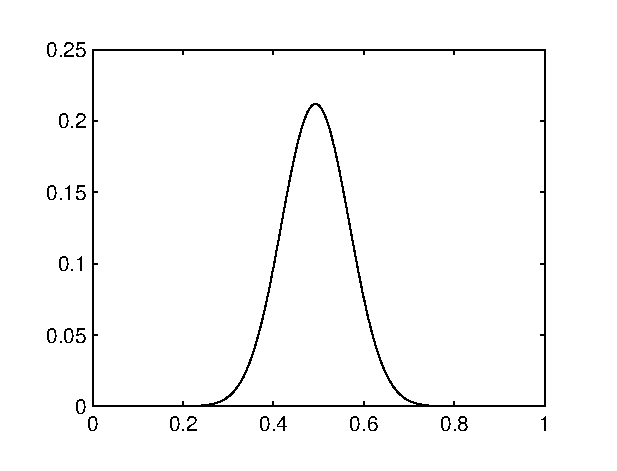
\includegraphics[width=\linewidth]{figures/espline_P15}
\caption{E-spline}
\end{subfigure}
\begin{subfigure}{.22\textwidth}
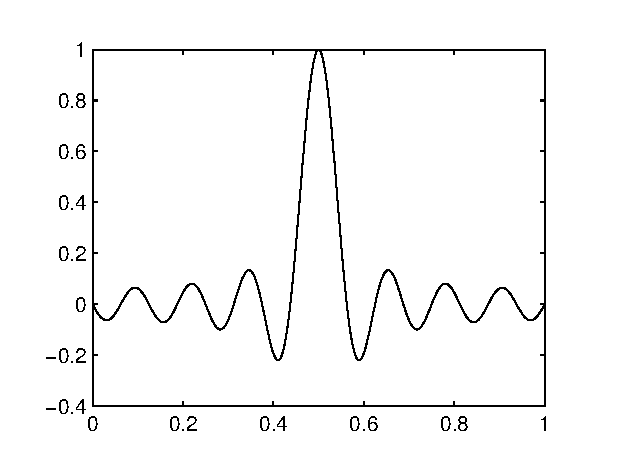
\includegraphics[width=\linewidth]{figures/modif_espline_P15}
\caption{Modified E-spline}
\end{subfigure}
\caption{Sampling kernels $h(t)=\varphi(-t/T)$ obtained from E-splines of order $P=15$ 
and scaled with $T=1/16$. Note that function $\varphi(t)$ is made anticausal in order
to have causal sampling kernels. 
%\red{The support of the E-splines is $L=P+1$, the sampling kernels in (a) and (b) 
%have a support of 1 due to the scaling factor.}
The modified E-spline (eMOMS) corresponds exactly to half period of the Dirichlet kernel of order $2(P+1)$.}
\label{fig:kernels}
\end{figure}

FRI theory \cite{vetterli2002,dragotti2005,dragotti2007,tur2011} shows that for a properly chosen filter $h(t)$, 
the signal $x(t)$ can be perfectly reconstructed from the samples $y_n$.
%Thus, the goal of the reconstruction scheme is to retrieve the $K$ pairs of unknowns $(t_k, a_k)$ 
%from the samples $y_n$.
We restrict our setup to exponential reproducing kernels \cite{dragotti2007}, which are functions 
that are able to reproduce exponentials:

\begin{equation}
\sum_{n \in \mathbb{Z}} c_{m,n} \; \varphi(t-n) = e^{\alpha_mt}, \quad m = 0,1, \ldots, P,
\label{eq:exp_kernel}
\end{equation}

\noindent
where $c_{m,n} \in \mathbb{C}$ and $\{\alpha_m\}_{m=0}^{P}$ are design parameters and are chosen
to be purely imaginary and in complex conjugate pairs in order to have a real valued
kernel $\varphi(t)$. More specifically, we use 
$\alpha_m =  j\tfrac{\pi}{P}(m-\tfrac{P}{2})$ for $m=0,\dots,P$.
There exist many functions of compact support in time that satisfy the 
exponential reproducing property \eqref{eq:exp_kernel}, such as for example E-splines \cite{dragotti2007} 
and the modified E-splines introduced in \cite{uriguen2011}. The latter, which are a variation 
of the maximal-order minimal-support kernels presented in \cite{blu2001}, 
are the exponential reproducing kernels that are most resilient to noise \cite{uriguen2011,uriguen2013}
and are the kernels of choice for our simulations. They are called eMOMS. 
Note that these kernels have support $P+1$.


In order to recover parameters $\left\lbrace t_k, a_k \right\rbrace_{k=1}^{K}$, first the samples 
$y_n$ are linearly combined with coefficients $c_{m,n}$ from \eqref{eq:exp_kernel}.
This leads to a new set of measurements 

\begin{equation}
s_m = \sum_{n \in \mathbb{Z}} c_{m,n} \; y_n, \quad m = 0, 1, \ldots, P.
\label{eq:s_m}
\end{equation}

\noindent
Combining \eqref{eq:y_n} and \eqref{eq:exp_kernel} it follows that $s_m$ can be expressed 
as a power sum series \cite{dragotti2007}:

\begin{equation}
s_m 
= \left\langle x(t) \, , \, e^{\alpha_m t / T} \right\rangle
= \sum_{k=1}^{K} b_k \, u_k^m,
\end{equation}

\noindent
where $b_k = a_k \, e^{\alpha_0 t_k / T}$ and $u_k = e^{j \pi t_k / PT}$.
The FRI recovery is thus turned into an amplitude and frequency estimation problem. 
This is a well-known problem in spectral analysis and can be solved, for instance, 
with the annihilating filter method \cite{stoica2005}. The critical number of measurements 
$s_m$ required to recover the $2K$ parameters $\left\lbrace t_k, a_k \right\rbrace_{k=1}^{K}$ 
is exactly $2K$ \cite{dragotti2007}. 
It thus follows that $P+1 \geq 2K$ in order to achieve perfect reconstruction.


\subsection{FRI reconstruction in the presence of noise}
\label{subsec:noise}
The solution explained so far is only ideal, since noise is generally present in the acquisition 
process. We assume the only source of noise $\varepsilon_n$ is added to the samples $y_n$. 
In addition, we consider $\varepsilon_n$ are i.i.d. Gaussian random variables, of zero mean and 
standard deviation $\sigma$. Thus, measurements \eqref{eq:s_m} become
$\tilde{s}_m = \sum_{n \in \mathbb{Z}} c_{m,n} \; (y_n + \varepsilon_n) = s_m + d_m$,
and alternative methods are needed to retrieve the pairs $(t_k,a_k)$. We may solve the problem 
by using the total least-squares method and Cadzow denoising algorithm \cite{cadzow1988} introduced 
for FRI in \cite{blu2008} or matrix pencil method \cite{hua1990} used for FRI in \cite{maravic2005}.
Further alternative methods can be found in \cite{tan2008,erdozain2011,berent2010}.


%\subsection{Samples $y_n$ influenced by $K$ Diracs}
%
%We have stated that we need at least $2K$ measurements $s_m$ to recover the time-delays and 
%amplitudes of the $K$ Diracs, but we have assumed that we have an infinite number of temporal 
%samples $y_n$ in \eqref{eq:s_m}. In what follows we analyse perfect reconstruction conditions with a finite 
%number of temporal samples.
%
%Consider we restrict the locations of the Diracs to a finite temporal interval, this is $t_k \in ]0, \tau]$, 
%and we use a sampling kernel of compact support, that is $\varphi(t) = 0$ for $t \notin [-L, 0]$
%~\footnote{Note that function $\varphi(t)$ is made anti-causal
%in order to have a causal sampling kernel $h(t) = \varphi(-t/T)$. The support of this kernel is $[0, LT]$.} 
%Thus, only a finite number of samples $y_n$ are non-zero. As shown by equation \eqref{eq:y_n}, 
%the samples $y_n$ correspond to the projection of the Diracs 
%onto scaled and shifted versions of $\varphi(t)$. Then, Diracs located in $]0, \tau]$ can only have an impact 
%on samples that correspond to indices $1 \leq n \leq \lfloor \tfrac{\tau}{T} + L\rfloor$ 
%(see Figure \ref{fig:sampling_interval}). 
%We can thus perfectly recover $K$ Diracs located in $]0,\tau]$ from a finite number of 
%samples $\lfloor \tfrac{\tau}{T} + L\rfloor$.


% Sequential sampling
% -------------------
\section{Sampling an infinite stream of Diracs}
\label{sec:inf_stream}

We now consider the case of an infinite train of Diracs 

\begin{equation}
x(t) = \sum_{k \in \mathbb{Z}} a_k \, \delta \left( t - t_k \right).
\label{eq:diracs_inf}
\end{equation}

\noindent
The signal $x(t)$ is assumed to have a finite local rate of innovation, 
as defined in \cite{vetterli2002}, of $2K/\tau$. This means that, 
if we consider a sliding window of size $\tau$, the number of Diracs 
that we see inside the window is always  at most $K$.
We propose a sequential algorithm that estimates the locations of the 
Diracs of \eqref{eq:diracs_inf} by using a sliding
window that sequentially covers the interval of time
\begin{equation} 
t \in \left] t_i, t_i + \tau \right].
\label{eq:tempInt}
\end{equation}

\noindent
The sliding window step is of $T$ seconds, which equals the sampling period.
%\red{as indicated in Figure \ref{fig:filter_n_sample} ($T < \tau$).}
We assume that $\tau$ is an integer multiple of $T$, specifically $\tau = NT$.
In what follows, we first establish some conditions on the number of samples $N$, the sampling period $T$ and
the order of the E-splines necessary to achieve perfect reconstruction of the infinite stream \eqref{eq:diracs_inf}. 
Second, we present a novel approach that is able to recover Diracs in high noise scenarios
processing the stream \eqref{eq:diracs_inf} sequentially.


\subsection{Noiseless case}

We analyze the ideal scenario in the first place to determine the conditions 
on the number of samples of the sliding window $N$, the sampling period $T$
and the support $P+1$ of the sampling kernel that allows our algorithm 
to be able to provide perfect reconstruction of \eqref{eq:diracs_inf}. In our 
approach we sequentially analyse sets of $N$ samples $y_n$ that cover the 
temporal interval \eqref{eq:tempInt}. 
%This corresponds to samples with indices $n = n_i + 1, \ldots, n_i + N$, where $t_i = n_i T$.
%To simplify the notation, and without loss of generality, we will present the analysis 
%for the simpler case $]0,\tau]$, and indices $n = 1, \ldots, N$.
Due to the fact that we consider a finite number of samples, there exist 
border effects that may stop us from achieving perfect reconstruction. 
%\red{This is illustrated in Figure \ref{fig:sampling_interval} for a window starting at $t_i=0$.}
The sampling kernel $\varphi(t/T)$ has compact support $(P+1)T$. Consequently, a Dirac influences 
$P+1$ samples. This means that a Dirac located just before the window of interest 
will generate non-zero samples that will leak inside 
the window. Moreover, a Dirac located at the end of the window of interest will 
generate non-zero samples beyond the $N$ samples we are considering and
therefore cannot be reconstructed. This is illustrated in Figure \ref{fig:border_effects}.

Since the algorithm operates sequentially we can assume that when operating on the window 
$t \in \left] t_i, t_i + \tau \right]$
we have already perfectly recovered Diracs up to the time instant $t_i$. Therefore 
their contributions can be removed and 
in this way we can overcome the border effect on the {\em left} of the window.

To overcome the border effect of the \textit{right}
side we determine certain conditions on the number of samples $N$,
the order $P$ of the kernel and the sampling period $T$. 
We have seen in Sec. \ref{sec:sampling} that exact recovery of $K$ Diracs requires
$P+1 \geq 2K$. 
Now, let us put ourselves in the worst case scenario, where we have $K$ Diracs evenly spaced 
with constant separation $\tau / K$. Each Dirac influences $P+1$ samples due to the support of the kernel.
Therefore, $K$ Diracs influence $K(P+1)$ samples $y_n$.
In this worst case scenario, we have to guarantee that $N \geq K (P+1)$ and combining this condition
with $P+1 \geq 2K$ we arrive at
%To be guaranteed that $K$ Diracs is at the end of the interval 
%for this scenario, we need to impose $\tfrac{\tau}{K} \geq (P+1)T$. Setting $\tau = NT$
%and combining this condition with $P+1 \geq 2K$ we arrive at

\begin{equation}
N \geq 2K^2.
\end{equation}

\begin{figure}[t]
\centering
\begin{subfigure}{.22\textwidth}
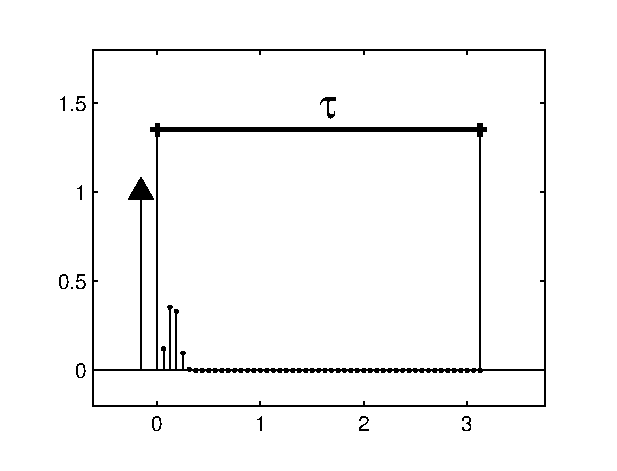
\includegraphics[width=\linewidth]{figures/border_effect_left}
\caption{}
\end{subfigure}
\begin{subfigure}{.22\textwidth}
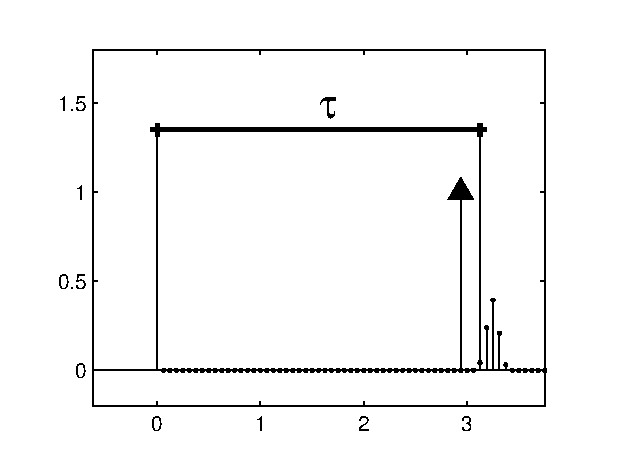
\includegraphics[width=\linewidth]{figures/border_effect_right}
\caption{}
\end{subfigure}
\caption{Border effects. (a) A nearby Dirac located before the observation window 
$\tau$ influences the samples $y_n$ of the window. (b) A Dirac inside the window 
but close to the right border generates non-zero samples outside the window.}
\label{fig:border_effects}
\end{figure}

As previously mentioned, when a Dirac is near the end of the interval, we are
not able to perfectly reconstruct it. The size of this area is $PT$.
Therefore, we can only perfectly recover $K$ Diracs when all of them are 
in a region of size $(N-P)T$. Again, in the case of constant separation $\tau / K$, 
we have to guarantee that there
will be a position of the sliding window such that the $K$ Diracs are in the perfect reconstruction area. 
Since they can occupy an interval of maximum size $(K-1) \tfrac{\tau}{K}$ and to 
make sure they are within the perfect reconstruction area for a certain window, we restrict this interval
to be smaller than or equal $(N-P-1)T$. Combining these conditions and choosing 
the smallest possible number of samples $N=2K^2$ we obtain

\begin{equation}
\begin{aligned}
(K-1) \frac{NT}{K} & \leq (N-P-1)T \\
\Leftrightarrow 
P                  & \leq 2K - 1.
\end{aligned}
\end{equation}

In addition, we know that $P$ has to satisfy $P \geq 2K - 1$. Consequently, we have that

\begin{equation}
{P=2K-1}.
\end{equation}

\noindent
The sampling period $T$ is given by the temporal interval $NT=\tau$ and
the number of samples $N \geq 2K^2$. We thus have $T \leq \tfrac{\tau}{2K^2}$.

The reconstruction algorithm processes the stream of samples sequentially, retrieving 
the locations of each set of maximum $K$ Diracs from $N$ samples by applying the annihilating filter method. 
Provided we satisfy the previously described conditions, all Diracs will 
be located in the perfect reconstruction interval of a certain position of the sliding window,
and thus recovered.
From the recovered Diracs of the current window, we recalculate
the $N$ samples that correspond to this window, and only if the reconstructed samples
are identical to the original ones, the Diracs are stored. 
The maximum number of Diracs $K$ within a window has to be estimated.
This is done by trying for all possible values of $K$, and only
when the correct value is estimated the reconstructed samples will coincide with the 
original ones. 

\subsection{Noisy scenario}

\begin{figure}[t]
\centering
\begin{subfigure}{.22\textwidth}
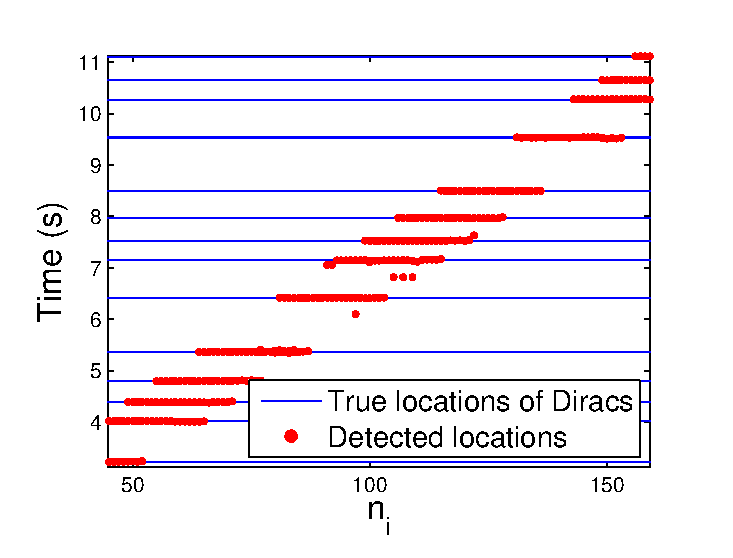
\includegraphics[width=\linewidth]{figures/noisy_scatter}
\caption{Retrieved locations}
\end{subfigure}
\begin{subfigure}{.22\textwidth}
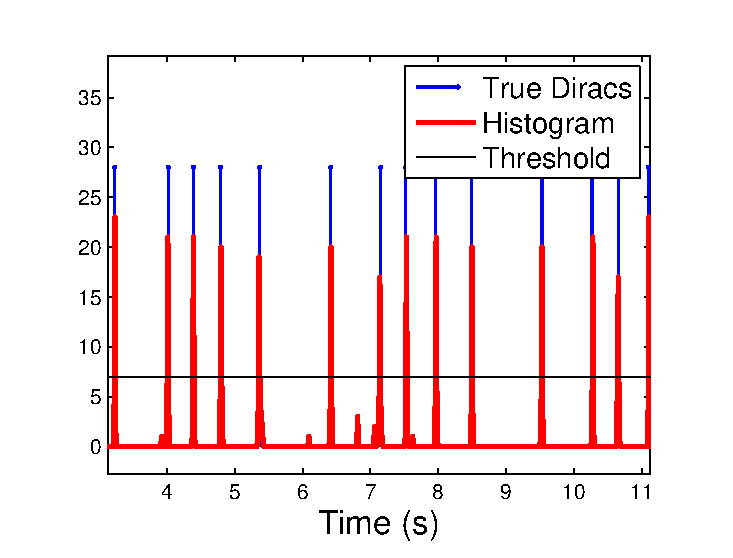
\includegraphics[width=\linewidth]{figures/noisy_histogram}
\caption{Locations histogram}
\end{subfigure}
\caption{Noisy scenario. (a) Plot of the sequentially retrieved locations, the horizontal 
axis indicates the index of the sliding window and the vertical axis the location in time.
(b) Histogram of the locations shown in (a). Horizontally aligned dots in (a) lead to peaks 
in the histogram in (b).}
\label{fig:noisy_locs}
\end{figure}

In the presence of noise, perfect reconstruction is not possible and the algorithm
previously described becomes unstable. Moreover, the strict conditions on $N$ and 
$P$ impose critical sampling, since we have exactly $2K$ values of the $s_m$ 
measurements to retrieve $K$ Diracs. In the noisy case we relax this condition and allow
higher values of $P$. This makes the denoising algorithms mentioned in Sec. \ref{subsec:noise}
more effective.

We thus develop a new strategy that is also based on using a sliding window 
and processing sets of $N$ samples in sequential order. 
For each window and each group of $N$ samples, we retrieve $K$ Diracs using the 
algorithm in Sec. \ref{sec:sampling} coupled with matrix pencil.
We then store  
all the locations and amplitude retrieved in that window. 
We then slide the window by $T$ and repeat the process.
When the found locations correspond to real Diracs, they will be consistent among 
different positions of the sliding window that capture these Diracs. 
Otherwise, locations that are not correct and correspond to noise will normally be not consistent.
For example, in Figure \ref{fig:noisy_locs}-(a) we plot the retrieved locations 
for different windows. The horizontal axis represents the index of the window corresponding to a retrieved location,
and the vertical axis the Dirac location in time. Consistent locations appear as horizontal alignments 
of dots, overlapping the blue lines.

In order to detect which locations are consistent, a second step is to construct a 
histogram of detected locations. Only the peaks of the histogram are assumed 
to correspond to real Diracs. For a peak in the histogram above a certain threshold, 
the location of the corresponding Dirac is estimated averaging all the retrieved
locations that contribute to this peak. This is illustrated in Figure \ref{fig:noisy_locs}-(b).

\begin{algorithm}
\footnotesize
\caption{Sequential FRI retrieval of Diracs}
\label{algo:sequential_fri}
\algsetup{indent=2em}
\begin{algorithmic}[1]
\REQUIRE $\left( y_n \right)_{n=1}^{N_{TOT}}$: stream of samples
\ENSURE  $\left\lbrace \left( t_k, a_k \right) \right\rbrace$: Dirac locations and amplitudes
\FOR{$n_i = 1$ to $N_{TOT}-N+1$} 
\STATE Retrieve $\left\lbrace \left( t_k^i, a_k^i \right) \right\rbrace$ 
from $\left( y_n \right)_{n=n_i}^{n_i+N-1}$
\ENDFOR
\STATE Construct histogram from retrieved locations $\left\lbrace t_k^i\right\rbrace$
\STATE Estimate Diracs from peaks of the histogram
\end{algorithmic}
\end{algorithm}


% Simulation results
% ------------------
\section{Simulation results}
\label{sec:simulations}

We have tested both versions of the algorithm: the noiseless case for which perfect
reconstruction is possible; and the noisy scenario, where locations are estimated from
the histogram of the retrieved locations. In the noiseless case we always perfectly
reconstruct the streams of Diracs with randomly generated locations and amplitudes. 
This is illustrated in Figure \ref{fig:perf_reconstr}. The stream of Diracs is 
generated to satisfy the maximum rate of $K$ Diracs per $\tau$ interval.

\begin{figure}[t]
\centering
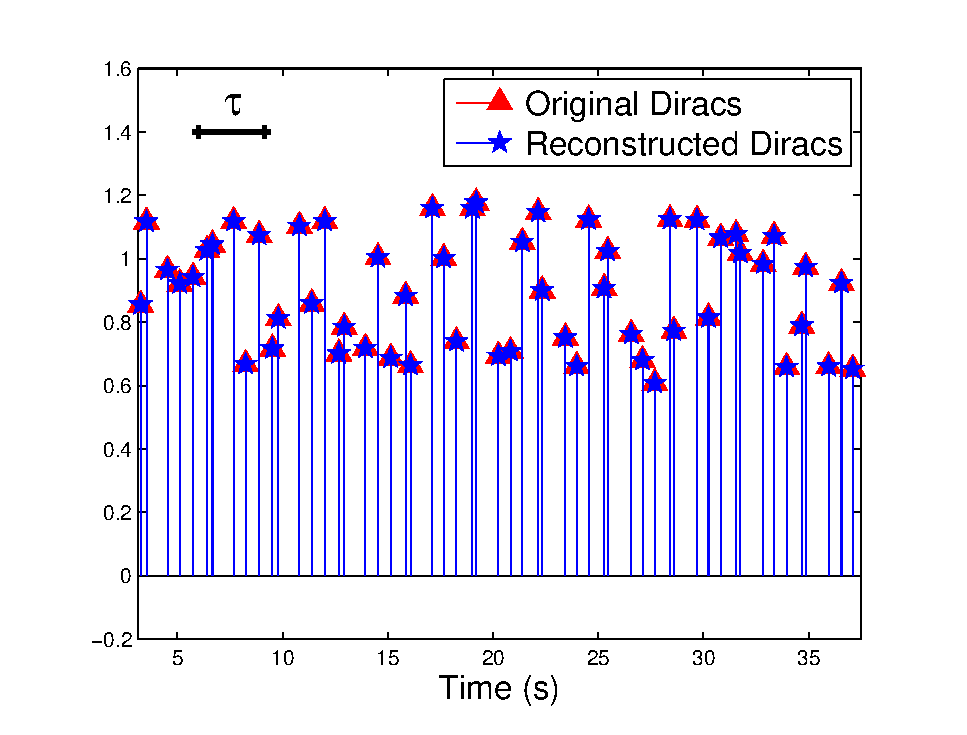
\includegraphics[width=.5\linewidth]{figures/diracs_perf_reconstr}
\caption{Sequential perfect reconstruction of a noiseless stream of 1000 Diracs with 10220 $y_n$ samples.
Only a small section of the stream is shown.
Rate $K=5$ Diracs per $\tau = 3.125$ s. $N=50$, $T=1/16$ and $P=9$. 
%\red{Even if $N=2K^2$ has to be 
%satisfied, this condition only holds locally for the sequential processing. 
%The total number of samples is much smaller than the square of the total number of Diracs.}
}
\label{fig:perf_reconstr}
\end{figure}

In the noisy scenario not all the Diracs are always
retrieved, and false positives may also happen. Note also that there is an uncertainty in 
the retrieved location. A retrieved Dirac is considered to correspond to a true Dirac if the difference 
between the real location and the estimated location is smaller than a threshold. Here we have 
set this threshold to $T/2$.
We randomly generate the locations of a stream of 1000 Diracs. We then take samples, 
contaminate them with noise and apply the sequential reconstruction algorithm. 
Figure \ref{fig:noisy_reconstr} shows one realisation of the procedure explained before.

\begin{figure}[t]
\centering
\begin{subfigure}{.22\textwidth}
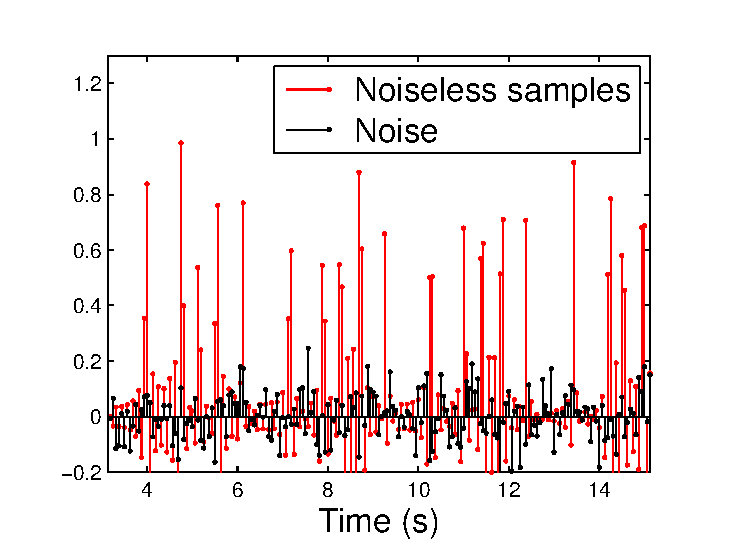
\includegraphics[width=\linewidth]{figures/noisy_samples}
\caption{$y_n$ samples}
\end{subfigure}
\begin{subfigure}{.22\textwidth}
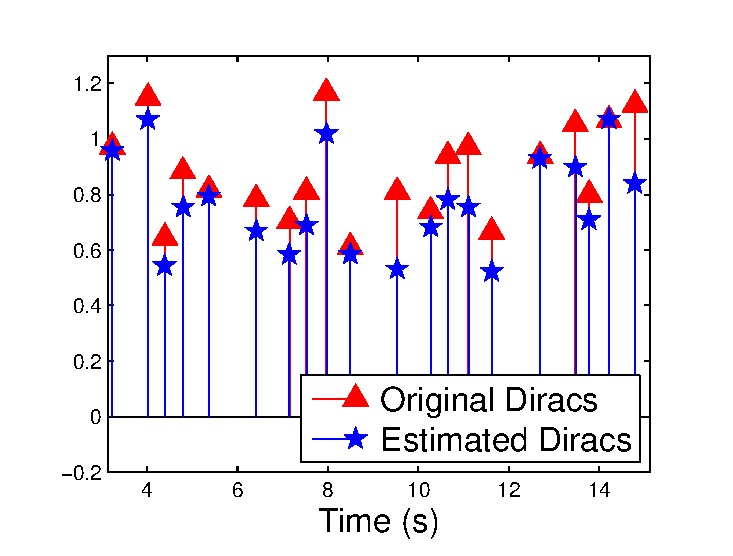
\includegraphics[width=\linewidth]{figures/noisy_reconstr}
\caption{Reconstructed stream}
\end{subfigure}
\caption{Noisy samples with a $\mathrm{SNR}=10$ dB and reconstructed stream 
from the peaks of the histogram of the retrieved locations. 
In all these simulations we used eMOMS as sampling kernel.}
\label{fig:noisy_reconstr}
\end{figure}

To further analyse the performance variation for different levels
of noise we run the algorithm over 100 different realisations of noise
for various levels of SNR. Table \ref{tab:results} summarises the obtained performances.

\begin{table}[h!]
\caption{Algorithm's performance. Stream of 1000 Diracs (630 seconds) and $10220$ 
samples, $T = 1/16$ s, $N = 50$, $P+1=23$. 
The detection rate is given in percentage of detected true Diracs. The
false positives are the average number of detected Diracs that do not correspond to true Diracs.
The precision is the standard deviation of the retrieved locations with respect to the true locations.}
\label{tab:results}
\begin{center}
\footnotesize
%\small
\begin{tabular}{|l|c|c|c|c|}
\hline 
SNR (dB)                     & 5         & 10        & 15        &   20      \\
\hline
\hline
Detection rate               & 97.69 \%  & 99.97 \%  & 100.00 \% & 100.00 \% \\
\hline
False positives              & 351.7     & 37.8      & 0.5       & 0.3       \\
\hline
Precision (s)                & 0.0086    & 0.0049    & 0.0028    & 0.0018    \\
\hline
\end{tabular}
\end{center}
\end{table}

The algorithm has been implemented in MATLAB and tested using a commercial laptop 
(2.5 GHz Intel Core i5 CPU). The average time required to process $10220$ samples 
corresponding to a stream of 630 seconds
containing 1000 Diracs
is about 105 seconds. 
%It is therefore possible to perform real-time reconstruction
%of very long streams of Diracs.


% Conclusions and future work
% ---------------------------
\section{Conclusions and future work}
\label{sec:conclusions}

In this paper we have presented a fast sequential algorithm to retrieve infinite streams
of Diracs in noiseless and noisy environments. 
In the noiseless case perfect reconstruction is achieved. In the noisy
scenario we propose to retrieve groups of $K$ Diracs sequentially and to retain only 
those Diracs whose locations have been consistently estimated in overlapping sliding windows.

We showed that the algorithm is able to process $10K$ samples in about $100$ seconds 
and can retrieve with high accuracy $1000$ Diracs even in very low SNR regimes.
%We are not aware of any current FRI algorithm able to achieve such performance for the same type of data.

\vfill\pagebreak

% Bibliography
% ------------
%\bibliographystyle{IEEEbib.bst}
\bibliographystyle{IEEEtran}
\bibliography{references}


% - end of content
% ------------------------------------------------------------------------------

\end{document}

% - end of document
% ------------------------------------------------------------------------------
